\chapter{Trilhas de estudo e projetos integradores}
\label{cap:projetos}

Já percorremos preparação, descrição, modelos e interpretação. Vamos agora organizar esses conhecimentos em projetos pequenos, que outra pessoa consiga abrir e compreender. A proposta é escolher perguntas, justificar caminhos e produzir uma narrativa dos resultados. Não precisamos executar todos os procedimentos disponíveis para mostrar que aprendemos.

Os dois primeiros projetos usam dados fictícios da apostila. O terceiro é uma atividade opcional com dados públicos do CNES. Em todos, vamos preservar os arquivos originais e separar o que foi planejado das explorações posteriores.

\section{Um roteiro comum e três entregáveis}

Antes de abrir uma análise, escreva a população ou o conjunto descrito, o significado de uma linha e a pergunta principal. Monte uma pasta com três entregáveis:

\begin{enumerate}
  \item \textbf{Projeto jamovi em \texttt{.omv}}: dados organizados, rótulos, transformações, filtros identificados e análises que respondem às perguntas escolhidas.
  \item \textbf{Dicionário de dados}: nome, significado, unidade, códigos, tipos de medida, ausentes e origem das variáveis calculadas. Registre também o significado da linha e da chave de identificação.
  \item \textbf{Relatório curto}: objetivo, fonte, preparação, método, estimativas, incerteza e limites. Selecione tabelas e figuras que sustentem a interpretação, em vez de reproduzir toda a saída.
\end{enumerate}

Salvar em CSV preserva valores, mas não substitui o projeto com suas análises; retome o capítulo~\ref{cap:manipulacao} e a documentação da planilha \parencite{JamoviPlanilha}. Como apoio, consulte o post \href{https://www.balaiocientifico.com/2024/04/salvar-e-exportar-dados-no-jamovi.html}{Salvar e exportar dados} e a \href{https://www.youtube.com/watch?v=tspLxfl3uZk}{Aula 4 do canal}.

\begin{figure}[H]
\centering
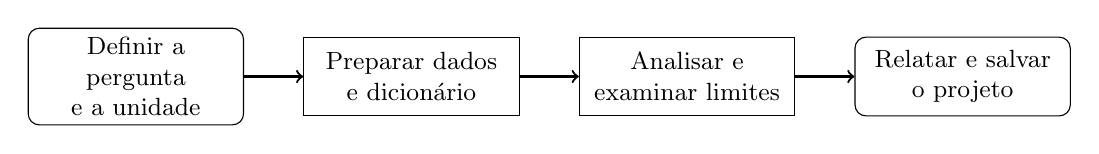
\begin{tikzpicture}[x=1cm,y=1cm,every node/.style={font=\small,align=center}]
  \node[draw,rounded corners,text width=2.5cm,minimum height=1cm] (p) at (0,0)
    {Definir a pergunta\\e a unidade};
  \node[draw,text width=2.5cm,minimum height=1cm] (d) at (3.5,0)
    {Preparar dados\\e dicionário};
  \node[draw,text width=2.5cm,minimum height=1cm] (a) at (7,0)
    {Analisar e\\examinar limites};
  \node[draw,rounded corners,text width=2.5cm,minimum height=1cm] (r) at (10.5,0)
    {Relatar e salvar\\o projeto};
  \draw[->,thick] (p)--(d);
  \draw[->,thick] (d)--(a);
  \draw[->,thick] (a)--(r);
\end{tikzpicture}
\caption{Um projeto conecta uma pergunta a decisões documentadas e resultados interpretáveis. O dicionário acompanha o processo. Elaboração própria.}
\label{fig:trilha-projeto}
\end{figure}

\section{Projeto 1: notas, comparações e modelos}

Abra \texttt{exemplo\_notas.csv}. Há 18 pessoas fictícias, cada uma com notas antes e depois, horas e uma atividade. Comece com frequências, médias, dispersões e gráficos por grupo, retomando o capítulo~\ref{cap:descritiva}. Confira os pares pelo identificador.

Escolha uma pergunta principal e uma extensão:

\begin{enumerate}
  \item \textbf{Leitura e Vídeo diferem na nota posterior?} Mantenha apenas esses grupos, documente o filtro e configure Welch conforme o capítulo~\ref{cap:hipoteses}. Relate a diferença e seu IC, com a orientação identificada.
  \item \textbf{Qual é a mudança média das mesmas pessoas?} Desative o filtro e trabalhe com \texttt{depois} menos \texttt{antes}, preservando os 18 pares. Não use um teste independente entre as duas colunas.
  \item \textbf{Como comparar as três atividades?} Desative o filtro Leitura/Vídeo e confirme as 18 pessoas nos três grupos. Use o capítulo~\ref{cap:anova} para distinguir a pergunta global das comparações específicas e explicitar a multiplicidade.
  \item \textbf{Como horas e nota anterior se relacionam com a nota posterior?} Ajuste o modelo do capítulo~\ref{cap:regressao}, examine os resíduos e compare a interpretação simples com a condicional.
\end{enumerate}

As quatro perguntas não são quatro tentativas para selecionar o menor valor de $p$. No relatório, explique por que escolheu suas análises. Identifique o caráter fictício e o tamanho pequeno do banco; uma mudança observada ou uma associação ajustada não demonstra eficácia causal.

Para revisar a preparação, use o post \href{https://www.balaiocientifico.com/2026/10/filtros-no-jamovi-selecionar-dados.html}{Filtros no jamovi}; para explorar relações, acompanhe a \href{https://www.youtube.com/watch?v=K507gYOjBMA}{Aula 15: gráfico de dispersão}. Entregue \texttt{projeto\_notas.omv}, o dicionário e um relatório com uma figura, uma tabela e conclusões nas unidades das notas.

\section{Projeto 2: pontuação, confiabilidade e dimensões}

Esta trilha tem duas partes com \textbf{bancos distintos}. Em \texttt{exemplo\_escalas.csv}, há 30 respostas fictícias a cinco itens ordinais; em \texttt{exemplo\_dimensoes.csv}, há 180 registros fictícios com oito indicadores contínuos. Identificadores de arquivos diferentes não representam pessoas correspondentes. Não empilhe nem una esses bancos para aumentar a amostra.

Na primeira parte, retome o capítulo~\ref{cap:confiabilidade}: confira limites, crie \texttt{item3\_corr}, calcule total e média e examine a consistência interna. Compare a pontuação antes e depois da correção para explicar o erro de direção, sem sugerir que a recodificação foi escolhida para melhorar o coeficiente. Consulte as opções oficiais de confiabilidade \parencite{JamoviConfiabilidade}.

Na segunda, siga o capítulo~\ref{cap:dimensoes}. Formule separadamente o objetivo de resumir variação por PCA e o de representar relações por AFE. Registre matriz utilizada, retenção, extração e rotação pertinentes; descreva cargas, unicidades e limites, sem apresentar os nomes das dimensões como validação do instrumento.

O post \href{https://www.balaiocientifico.com/2026/10/como-criar-uma-variavel-calculada-no.html}{Variável calculada: soma e média} e a \href{https://www.youtube.com/watch?v=NBvQphd9FqI}{Aula 9: calculadora de variáveis} apoiam a preparação dos escores. Salve dois projetos \texttt{.omv}, dois dicionários e um relatório comparativo. A conclusão deve distinguir pontuação, consistência e estrutura, preservando a origem de cada resultado.

\section{Projeto 3: uma descrição documentada do CNES}

Vamos escolher uma competência mensal e um recorte territorial para descrever estabelecimentos ou vínculos profissionais. Comece pelo post \href{https://www.balaiocientifico.com/2025/04/analise-de-dados-do-cnes-no-jamovi.html}{Análise de dados do CNES no jamovi}, pelo vídeo de \href{https://www.youtube.com/watch?v=yp9d8hDmsew}{obtenção dos arquivos} e pelo de \href{https://www.youtube.com/watch?v=0Jcaehp7f8Y}{importação e dicionário}. Confira formatos e definições na \href{https://cnes.datasus.gov.br/pages/downloads/documentacao.jsp}{documentação oficial do CNES} e obtenha os arquivos no \href{https://cnes.datasus.gov.br/pages/downloads/arquivosBaseDados.jsp}{portal oficial}.

\subsection{A unidade vem antes da contagem}

Um registro de estabelecimento e um registro de vínculo profissional respondem a perguntas distintas. A mesma pessoa pode estar ligada a mais de um estabelecimento; linhas de vínculos não são automaticamente pessoas únicas. A \href{https://wiki.saude.gov.br/cnes/index.php/Como_cadastrar_um_profissional_no_CNES}{orientação oficial de cadastro profissional} distingue identificação e vínculos.

\begin{figure}[H]
\centering
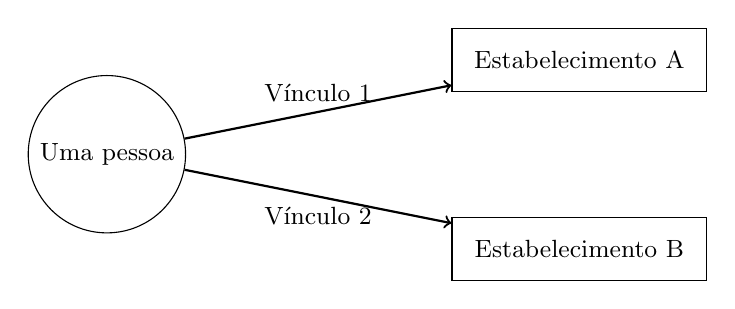
\begin{tikzpicture}[x=1cm,y=1cm,every node/.style={font=\small,align=center}]
  \node[draw,circle,minimum size=1.6cm] (p) at (0,0) {Uma pessoa};
  \node[draw,text width=3cm,minimum height=0.8cm] (e1) at (6,1.2) {Estabelecimento A};
  \node[draw,text width=3cm,minimum height=0.8cm] (e2) at (6,-1.2) {Estabelecimento B};
  \draw[->,thick] (p) -- node[above] {Vínculo 1} (e1);
  \draw[->,thick] (p) -- node[below] {Vínculo 2} (e2);
\end{tikzpicture}
\caption{Esquema hipotético: uma pessoa vinculada a dois estabelecimentos. Contar os dois vínculos como duas pessoas mudaria a unidade da pergunta. A estrutura concreta deve ser conferida no dicionário do arquivo. Elaboração própria.}
\label{fig:cnes-unidades}
\end{figure}

\subsection{Receita de preparação e relato}

\begin{enumerate}
  \item Registre endereço da fonte, nome do arquivo, data de obtenção, competência e território. A competência do dado não é a data em que ele foi baixado.
  \item Leia o dicionário, preserve códigos de identificação e confira delimitador, decimais, ausentes e rótulos. Não transforme código territorial em quantidade contínua.
  \item Defina a chave compatível com o arquivo. Investigue repetições antes de remover linhas: elas podem representar vínculos ou competências diferentes.
  \item Produza uma tabela descritiva e um gráfico. Explicite se o denominador é estabelecimento, vínculo ou outra unidade definida. Uma tabela de contingência pode apoiar a organização, como no capítulo~\ref{cap:categoricos}.
\end{enumerate}

Um percentual por tipo deve declarar o conjunto elegível: $100\times N_{\mathrm{tipo}}/N_{\mathrm{elegivel}}$. Contagem de vínculos não é taxa populacional; uma taxa exige um denominador populacional e período compatíveis. Não interprete cadastro como atendimentos realizados ou cobertura efetiva sem informações adicionais.

Entregue o \texttt{.omv} do recorte analisado, dicionário e relatório com a fonte e as decisões de inclusão. O objetivo é uma descrição verificável, sem números atuais predefinidos nem testes inferenciais automáticos sobre todo o cadastro.

\section{Vamos praticar: perguntas e comentários}

\begin{enumerate}
  \item Duas colunas antes/depois das mesmas pessoas justificam um teste independente?
  \item Podemos unir os dois bancos do projeto 2 pelo identificador para estudar confiabilidade e dimensões juntos?
  \item Por que 100 linhas de vínculos do CNES não demonstram a presença de 100 profissionais diferentes?
  \item Qual informação precisa acompanhar uma porcentagem para permitir sua interpretação?
\end{enumerate}

\subsection*{Comentários das respostas}

\begin{enumerate}
  \item Não. A ligação entre medidas define pares; a escolha acompanha a pergunta sobre mudança e suas condições.
  \item Não. São conjuntos fictícios distintos. Use arquivos e dicionários separados e compare as perguntas e procedimentos no relatório.
  \item Uma pessoa pode contribuir com mais de um vínculo; a estrutura, a competência e a chave precisam ser verificadas antes da contagem.
  \item O numerador, o denominador elegível, a unidade, o recorte e, quando pertinente, o período. O símbolo de porcentagem sozinho não informa a população descrita.
\end{enumerate}
